
Manually assigning topics can be an error-prone activity that can lead to
wrongly specified terms. Literature is plenty of several approaches that mine and exploit available data to analyze repositories. Nevertheless, few of them cope with the topic recommendation task, which can be crucial in the project's development initial phase. Figure \ref{fig:spark} shows an example repository with related topics. By this simple snapshot, a \GH user can figure out that the \emph{apache spark} project makes usage of several programming languages such as \emph{java, r,} and \emph{python} to analyze \emph{big-data} and databases by exploiting common techniques used in this domain \ie \emph{sql and jdbc}. 

\begin{figure*}[h!]
	\centering
	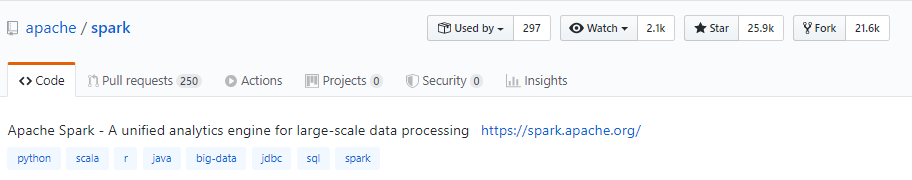
\includegraphics[width=0.8\linewidth]{figs/spark_topics.png}
	\caption{Example of a \GH repository and its topics.}
	\label{fig:spark}
\end{figure*}

As mentioned before, the \MNB using the \RM file of a repository to predict featured topics. It involves all the standard techniques employed in the ML domain \ie textual engineering, feature extraction, and training phase. By relying on the multinomial probability distribution, the approach is able to extract relevant information from the \RM file and suggest a set of topics. Table \ref{tab:example} shows an example of the \MNB's outcomes given the list of the actual repository topics. 

\begin{table}[h]
\centering

\resizebox{8.5cm}{!} {

\begin{tabular}{| p{3.2cm} | p{3.2cm} | }
\hline
 \textbf{Actual Topics} &\textbf{ Predicted topics} \\ \hline
     python,blender-scripts, spaceship, procedural-generation, game-development, 3d        &  
  shell, terminal, \textbf{3d},	opengl,	\textbf{python}        \\ \hline

\end{tabular}
}
\caption{Example of the \MNB outcomes.}
\label{tab:example}
\end{table} 


Even though the \MNB works in practice, it suffers from some limitations. First, the underlying model can recommend only featured topics that represent only a small set of all possible terms. In this way, the \MNB doesn't express all the concepts covered by a \GH repository. As shown in the table, only two of the predicted topics matched with the real ones. The second major limitation is the underlying structure needed for the training phase. To deliver relevant items, the \MNB requires a \emph{balanced} dataset, \ie each topic must have a similar number of  \RM files. This scenario is difficult to meet in reality as the topics' heterogeneity is extremely high. Furthermore, the \GH platform is regularly updated with new projects and, consequently, with new topics. Thus, the training phase must take place several times to avoid outdated recommendations. 